\section{Results}
\label{sec:results}

All numbers below are generated by \texttt{scripts/summarize.py} from per-run logs.
Unless noted, they are \PD-test top-1 accuracies, given as mean $\pm$ std over three seeds.
``Paired $\Delta$'' is the seed-averaged difference between two configurations, with a paired 95\% bootstrap CI over \PD test images (\cref{tab:paired}).

\begin{table*}[t]
\centering\small
\begin{tabular}{lcccccc}\toprule
Model & PV & PD & PD$_\text{dedup}$ & PD F1 & Gap & CI$_{95}$ \\\midrule
MobileNetV3-L & 98.9 $\pm$ 0.1 & 30.9 $\pm$ 1.9 & 31.1 $\pm$ 2.2 & 27.6 $\pm$ 0.6 & 67.9 $\pm$ 1.9 & 6.0 \\
EfficientNet-B0 & 99.4 $\pm$ 0.0 & 31.9 $\pm$ 2.4 & 32.5 $\pm$ 2.5 & 28.0 $\pm$ 1.2 & 67.5 $\pm$ 2.4 & 5.9 \\
DINOv2 ViT-S/14 (linear probe) & 97.6 $\pm$ 0.1 & 46.2 $\pm$ 1.7 & 46.6 $\pm$ 0.7 & 44.3 $\pm$ 2.0 & 51.4 $\pm$ 1.7 & 6.2 \\
DINOv2 ViT-S/14 (fine-tune) & 99.5 $\pm$ 0.1 & 37.7 $\pm$ 2.2 & 38.1 $\pm$ 1.8 & 36.1 $\pm$ 1.9 & 61.8 $\pm$ 2.3 & 6.3 \\
CLIP ViT-B/32 (zero-shot) & 25.2 & 29.2 & 28.7 & 24.6 & -4.0 & -- \\
\bottomrule\end{tabular}

\caption{\textbf{Trained on \PV only} (28 classes, no field labels). PV = in-domain \PV leaf-grouped test top-1; PD = \PD test top-1; PD$_\text{dedup}$ = \PD test with \PDdups near-duplicates of \PD-train removed; PD F1 = macro-F1 over the 27 classes present; Gap = PV$-$PD; CI$_{95}$ = average half-width of the per-run 95\% bootstrap interval on PD. Mean $\pm$ std over 3 seeds.}
\label{tab:source}
\end{table*}

\paragraph{The lab-to-field gap is large and universal (C1 holds).}
Every model reaches 97.6--99.5\% on the leaf-grouped \PV test split, and every model loses between \dinovtwoslpGap\ and \mnvthreeGap\ points on \PD (\cref{tab:source}).
Both edge CNNs land near 31\%, which is close to CLIP zero-shot (\ClipPD\%) even though CLIP never saw a single disease label.
Removing the \PDdups near-duplicate test images moves the source-only numbers by less than one point, as expected: these models never saw \PD training images.

\paragraph{Generic self-supervised features transfer best, if left frozen (C2 holds).}
A linear probe on frozen DINOv2 ViT-S features trained only on \PV reaches \dinovtwoslppvpre\% on \PD, \PCa\ points above EfficientNet-B0 (paired 95\% CI [\PCalo, \PCahi]).
Fine-tuning the same backbone on \PV \emph{raises} in-domain accuracy (\dinovtwosftPVin\% vs.\ \dinovtwoslpPVin\%) but \emph{lowers} field accuracy: the frozen probe is ahead by \PCb points (paired CI [\PCblo, \PCbhi]).
This is consistent with fine-tuning on a narrow, uniform-background source eroding general features that transfer to clutter. Our runs do not isolate that mechanism.

\begin{figure*}[t]
\centering
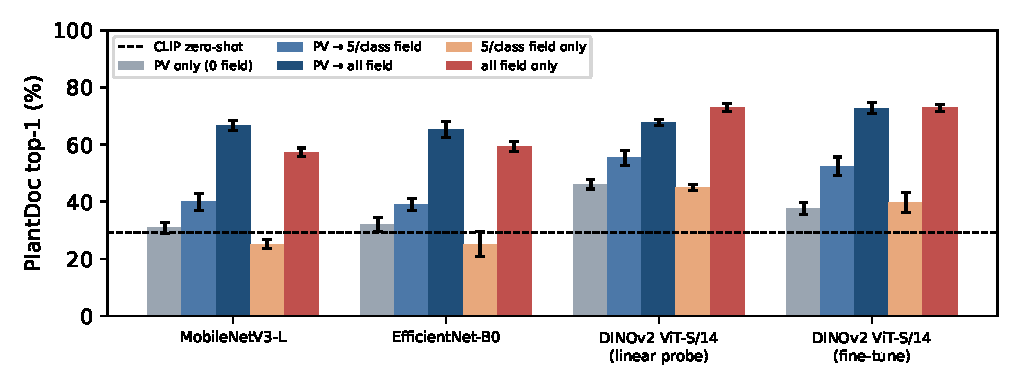
\includegraphics[width=0.66\linewidth]{../results/figures/field_labels.pdf}\hfill
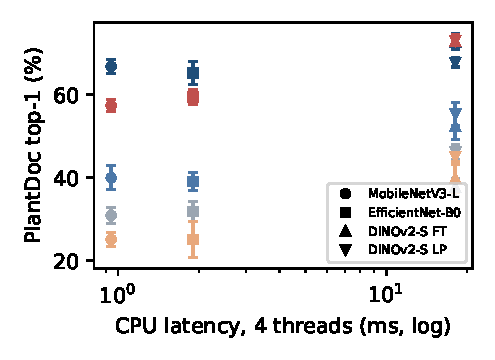
\includegraphics[width=0.32\linewidth]{../results/figures/acc_vs_latency.pdf}
\caption{\textbf{Left:} \PD top-1 by model and label regime (mean $\pm$ std over 3 seeds; dashed line: CLIP zero-shot). \textbf{Right:} the same points against measured CPU latency (ONNX Runtime, 4 threads, batch 1, log scale). Colors match the left panel. Latency for the linear probe equals that of the fine-tuned ViT.}
\label{fig:labels}
\end{figure*}

\begin{table*}[t]
\centering\small
\begin{tabular}{lccccc}\toprule
Model & PV only (0 field) & PV $\rightarrow$ 5/class field & PV $\rightarrow$ all field & 5/class field only & all field only \\\midrule
MobileNetV3-L & 30.9 $\pm$ 1.9 & 40.0 $\pm$ 2.9 & 66.8 $\pm$ 1.8 & 25.1 $\pm$ 1.6 & 57.3 $\pm$ 1.5 \\
EfficientNet-B0 & 31.9 $\pm$ 2.4 & 39.1 $\pm$ 2.1 & 65.3 $\pm$ 2.8 & 25.1 $\pm$ 4.3 & 59.5 $\pm$ 1.8 \\
DINOv2 ViT-S/14 (linear probe) & 46.2 $\pm$ 1.7 & 55.4 $\pm$ 2.7 & 67.8 $\pm$ 1.1 & 45.1 $\pm$ 1.1 & 73.0 $\pm$ 1.4 \\
DINOv2 ViT-S/14 (fine-tune) & 37.7 $\pm$ 2.2 & 52.4 $\pm$ 3.3 & 72.7 $\pm$ 2.0 & 39.8 $\pm$ 3.5 & 72.9 $\pm$ 1.1 \\
\bottomrule\end{tabular}

\caption{\textbf{\PD top-1 vs.\ field labels.} ``PV$\rightarrow$'' starts from the \PV-trained model of the same seed. ``only'' starts from generic pretrained weights. Mean $\pm$ std over 3 seeds. The de-duplicated variant is in \texttt{results/summary.md}.}
\label{tab:labels}
\end{table*}

\paragraph{Lab models fail first at recognizing the crop.}
Because each class is a (crop, condition) pair, we can split errors into two kinds (\cref{tab:errors}).
Lab-trained CNNs pick the wrong \emph{crop} for nearly half of the field images (crop accuracy \CropAccMnv--\CropAccEff\%). Given the right crop, they pick the exact class only \ClassGivenCropEff--\ClassGivenCropMnv\% of the time.
Most of the frozen DINOv2 probe's advantage is in crop recognition (\CropAccLP\%). Its class accuracy given the right crop (\ClassGivenCropLP\%) is close to the CNNs'.
Healthy-vs.-diseased accuracy is 82--87\% for lab-only models, against a majority-class baseline of \HealthyMajority\%.
In other words, the field failure is not only about subtle lesion appearance. Lab models also fail to recognize the plant itself in cluttered scenes.
This analysis was added after the main results were in, so it is exploratory.

\begin{table}[t]
\centering\scriptsize\setlength{\tabcolsep}{3pt}
\resizebox{\linewidth}{!}{\begin{tabular}{llccc}\toprule
Model & Regime & Crop & Class$\mid$crop & Healthy? \\\midrule
MobileNetV3-L & PV only & 53.8 & 57.5 & 83.9 \\
MobileNetV3-L & PV$\rightarrow$all & 83.9 & 79.6 & 94.9 \\
EfficientNet-B0 & PV only & 55.9 & 57.2 & 82.3 \\
EfficientNet-B0 & PV$\rightarrow$all & 83.8 & 77.9 & 93.4 \\
DINOv2 (linear probe) & PV only & 74.6 & 61.9 & 86.9 \\
DINOv2 (linear probe) & PV$\rightarrow$all & 90.1 & 75.2 & 93.2 \\
DINOv2 (fine-tune) & PV only & 64.8 & 58.2 & 84.5 \\
DINOv2 (fine-tune) & PV$\rightarrow$all & 91.0 & 80.0 & 96.0 \\
\bottomrule\end{tabular}
}
\caption{\textbf{Error decomposition on \PD test} (mean over 3 seeds, \%). Crop: predicted crop is correct. Class$\mid$crop: exact class correct among images with the correct crop. Healthy?: healthy-vs.-diseased correct (majority baseline \HealthyMajority\%).}
\label{tab:errors}
\end{table}

\paragraph{Five field images per class are not enough (C3 falsified).}
With 5 \PD images per class on top of \PV training, accuracy rises by 7--15 points (\cref{tab:labels}, \cref{fig:labels}). That recovers only \effbzeroRec\% (EfficientNet-B0), \mnvthreeRec\% (MobileNetV3) and \dinovtwoslpRec\% (both DINOv2 variants) of the gap between PV-only and PV$\rightarrow$all. This falls short of the 50\% we pre-registered.
For a practitioner, a few labeled field photos per disease help, but they are not a substitute for a real field training set.

\paragraph{Whether lab data helps depends on the model and the label budget.}
In the 5-per-class regime, starting from \PV is clearly better for every model, by +10 to +15 points (\cref{tab:paired}).
With all \PD training labels, \PV pretraining still helps both CNNs (MobileNetV3 \PCe, EfficientNet-B0 \PCg\ points). It makes no difference for fine-tuned DINOv2 (\PCk, CI [\PCklo, \PCkhi]), and it \emph{hurts} the frozen DINOv2 probe (\PCi, CI [\PCilo, \PCihi]).
For the probe, the explanation is narrow by construction. Its backbone is frozen and identical in both arms, so \PV enters \emph{only} through the starting point of the linear head. A head fitted to lab images is a useful prior when field labels are scarce (+10 points at 5/class). With all field labels, under our fixed schedule of 15 epochs, it ends up worse than a freshly initialized head.
For fine-tuned DINOv2, where the backbone does change, \PV pretraining is neutral once all field labels are available.
The best \PD accuracy overall (\dinovtwoslppdallpre\%) comes from the frozen DINOv2 probe trained on field data alone.

\begin{table}[t]
\centering\scriptsize\setlength{\tabcolsep}{2pt}
\resizebox{\linewidth}{!}{\begin{tabular}{lcc}\toprule
Comparison (A vs.\ B) & A$-$B & 95\% CI \\\midrule
DINOv2-LP vs EfficientNet-B0 (PV only) & +14.3 & [+8.2, +20.2] \\
DINOv2-LP vs DINOv2-FT (PV only) & +8.5 & [+3.1, +13.6] \\
DINOv2-LP (PV only) vs CLIP zero-shot & +16.9 & [+8.1, +25.3] \\
MobileNetV3-L: PV$\rightarrow$5/class vs 5/class only & +14.8 & [+10.7, +19.1] \\
MobileNetV3-L: PV$\rightarrow$all vs all field only & +9.5 & [+5.6, +13.3] \\
EfficientNet-B0: PV$\rightarrow$5/class vs 5/class only & +14.0 & [+10.2, +17.9] \\
EfficientNet-B0: PV$\rightarrow$all vs all field only & +5.8 & [+2.3, +9.3] \\
DINOv2 (linear probe): PV$\rightarrow$5/class vs 5/class only & +10.3 & [+5.6, +14.8] \\
DINOv2 (linear probe): PV$\rightarrow$all vs all field only & -5.2 & [-8.8, -2.0] \\
DINOv2 (fine-tune): PV$\rightarrow$5/class vs 5/class only & +12.6 & [+8.3, +16.9] \\
DINOv2 (fine-tune): PV$\rightarrow$all vs all field only & -0.1 & [-3.1, +3.0] \\
\bottomrule\end{tabular}
}
\caption{\textbf{Paired comparisons} on \PD test (seed-averaged top-1 difference in points, A$-$B; 95\% paired bootstrap CI over test images, 5{,}000 resamples, no multiple-comparison correction). LP/FT = DINOv2 linear probe / fine-tune.}
\label{tab:paired}
\end{table}

\paragraph{Edge cost (C4 falsified).}
\cref{tab:edge} reports cost on a desktop CPU (\EdgeCPU) and the RTX 5080.
The CNNs run in about 1--2\,ms per image with 4 CPU threads; DINOv2 ViT-S needs \CPUfourDino\,ms (\CPUoneDino\,ms single-threaded) and is about $5\times$ larger.
Our pre-registered C4 asked for a configuration within 5 points of the best accuracy at under 15\,ms. No configuration meets it. The fast CNNs peak at \mnvthreepdallinit\% (MobileNetV3, PV$\rightarrow$all), just below the 68.0\% threshold. The accurate DINOv2 models narrowly miss the latency limit, and the gap would widen on actual field hardware.
In practice the trade-off is mild in absolute terms: MobileNetV3 gives up about 6 points relative to the best model, in exchange for roughly $20\times$ lower CPU latency.

\begin{table}[t]
\centering\scriptsize\setlength{\tabcolsep}{2pt}
\resizebox{\linewidth}{!}{\begin{tabular}{lcccccc}\toprule
Model & Params (M) & ONNX (MB) & CPU-1 (ms) & CPU-4 (ms) & GPU (ms) & GPU mem (MB) \\\midrule
MobileNetV3-L & 4.2 & 16.1 & 2.7 & 0.9 & 3.53 & 40 \\
EfficientNet-B0 & 4.0 & 15.3 & 5.3 & 1.9 & 4.21 & 40 \\
DINOv2 ViT-S/14 & 21.6 & 82.4 & 51.8 & 18.1 & 2.76 & 139 \\
\bottomrule\end{tabular}
}
\caption{\textbf{Inference cost} at batch 1, $224\times224$: median over 300 runs after 50 warm-up runs. CPU: ONNX Runtime with 1 or 4 threads. GPU: PyTorch bf16. Params include the 28-way head.}
\label{tab:edge}
\end{table}

\paragraph{Seed noise vs.\ test noise (C5 holds, narrowly).}
Seed std on \PD reaches \effbzeroSeedSD\ points (EfficientNet-B0), just above our 2-point threshold. The per-run bootstrap interval half-width (\CIhwMin--\CIhwMax\ points) is about three times larger.
Seed averaging therefore stabilizes \emph{model} estimates, but it cannot fix a 236-image test set. Comparisons that differ by less than about 5 points on this split should be treated as ties unless a paired test says otherwise.
